%RMS SMALL SIGNAL STABILITY

\subsubsection{Power system stability}

Power system stability is defined as that property of a power system that enables it to 
remain in a state of operating equilibrium under normal conditions and to regain an acceptable 
state of equilibrium after being subjected to a disturbance \cite{StabilityAndControlKundur}. Other definitions
state not only the state of equilibrium must be acceptable but also most system variables must be 
bounded so that practically the entire system remains intact\cite{KundurDef}.


Although the primary concern is the behavior of the interconnected system as a whole, the stability of individual
components such as generators, motor loads, or regional subsystems; can be equally significant, particularly when 
localized instability does not propagate to the broader network. The system's dynamic behavior is governed by nonlinear 
interactions among its elements, and its response to perturbations is influenced by both the prevailing operating conditions
and the specific nature of the disturbance. Stability is understood around an equilibrium point and is subject to change
under small or large disturbances.

Power system stability is commonly classified depending on the physical nature of the instability, the size of the disturbance 
considered and the devices, processes and time span that must be considered to assess stability \cite{KundurDef}.
The combination of these factors influence the methodologies, tools and considerations used in the analysis. The main categories of power system stability are 
described in the following enumeration.

\begin{itemize}
    \item \textit{Rotor angle stability}: The ability the ability of the interconnected synchronous machines in a power system 
    to remain in synchronism under normal operating conditions and to regain synchronism after being subjected to a
     small or large disturbance \cite{StabilityAndControlKundur}. A synchronous machine stays in synchronism when the 
     electromagnetic torque exactly balances the mechanical torque from the prime mover, producing zero net accelerating torque. 
     Stability therefore depends on the machine and its controls restoring that torque balance after a disturbance; failure to do 
     so causes rotor acceleration or deceleration and loss of synchronism.
    \item \textit{Voltage stability}: The capacity of the network to maintain acceptable voltage magnitudes at all buses 
    during normal operation and following disturbances, such that voltages do not decrease sustainedly. Loss of this 
    capacity manifests as progressive voltage drops and, ultimately, voltage collapse, which may force extensive load disconnection 
    or generalized service interruption.
    \item \textit{Frequency stability}: The capability of the system to preserve a near-nominal frequency following a major 
    imbalance between generation and demand, through inertial response and secondary/tertiary control actions. Inadequate frequency 
    stability results in sustained under-frequency or over-frequency transients that can damage equipment, trigger protective disconnections, 
    and precipitate broader system failure.
\end{itemize}

Due to the increasing penetration of power electronics into the grid, two new categories of stability have been considered \cite{DefStabExtended}.

  
\begin{itemize}
    \item \textit{Converter-driven stability}: Refers to oscillatory behavior caused by control interactions in converter-interfaced generation (CIG). 
    Fast-interaction instabilities arise from high-frequency dynamics (hundreds of Hz to kHz) involving inner control loops and grid components. 
    Slow-interaction instabilities occur at low frequencies (<10 Hz), driven by PLL and outer-loop controls, especially 
    in weak grids. Synchronization issues and power transfer limits further compromise stability. 
    These phenomena differ from classical generator dynamics and require tailored mitigation strategies
    \item \textit{Resonance stability}: Refers to the system's ability to withstand oscillatory 
    energy exchange without magnifying voltage, current, or torque beyond safe limits. It includes subsynchronous 
    resonance (SSR), which arises from interactions between series compensation and either mechanical shaft modes or 
    electrical generator characteristics. The mechanical form leads to torsional resonance, while the electrical 
    form—9 (Induction Generator Effect (IGE)) can cause self-excitation. Converter controls in DFIGs can exacerbate these 
    effects, leading to subsynchronous control interaction (SSCI). These phenomena pose risks to both mechanical integrity 
    and electrical equipment.
\end{itemize}


Rotor angle stability is inherent of classical power systems with synchronous machines. Modern power grids, with the increasing penetration of 
power electronics, have introduced new dynamics and interactions that can affect rotor angle stability. Converters decrease the inertia of the system
and have an effect on the electromechanical modes. However, the fundamental principles of rotor angle stability remain intact and still takes
a crucial role on stability analysis of power systems.

Therefore, understanding and analyzing rotor-angle stability remains essential for ensuring the overall reliability of power systems. 
Insufficient or negative synchronizing torque produces aperiodic, non-oscillatory transient instability that drives large rotor-angle deviations
and is typically studied with time-domain numerical integration. In contrast, the absence of adequate damping torque gives rise to small-disturbance
oscillatory instability.

In the context of this thesis, the focus is on rotor angle stability, particularly small-signal stability, its eigenvalue-based characterization, 
modal properties, and analysis methods. The following sections describe the theoretical background and methodologies used for small-signal stability 
analysis in power systems. 

\subsubsection{Stability of a dynamic system}

A dynamic system is considered stable if, when subjected to a disturbance, it returns to its original state or to a new equilibrium state without
exhibiting unbounded behavior. The equilibrium points are those states where all the derivatives $\dot{x}$ are zero, meaning the system is at rest
or in a steady state. 

Linearity affects on the stability of a system. The stability of a liner system is independent of the input and the initial conditions.
However, for a non-linear system, stability depends on the magnitude of the input and initial conditions. Depending on the region of the state-space,
stability is classified into the following categories:

\begin{itemize}
  \item \textit{Local stability}: the system is locally stable around an equilibrium point if when a small perturbation is applied,
  it remains around the equilibrium point. If as time increases it returns to the equilibrium point, it is locally asymptotically stable\cite{StabilityAndControlKundur}.
  \item \textit{Finite stability}: the system is finitely stable if when a perturbation of finite size is applied, it remains bounded and does not diverge to infinity.
  \item \textit{Global stability}: the system is globally stable if it returns to an equilibrium point for any initial condition in the whole state-space.
\end{itemize}

Therefore, linearizing a non-linear system around an equilibrium point allows to study its local stability as if it was a linear system. 

\subsubsection{Small-signal stability}

Small-signal stability refers to the ability of a power system to maintain synchronism when subjected to 
small disturbances \cite{StabilityAndControlKundur}, such as minor load changes or small faults. These small disturbances
(typically within 1\%)occur frequently in power systems and allow the linearization of non-linear system equations
 around a specific operating point in order to perform analysis. The resulting linear representation enables the use
  of standard control engineering tools to assess system stability and dynamic performance \cite{SmallSignalCheah}.

The resulting instability due to those small perturbations can have two forms: Non-oscillatory unstability defined as an 
increase in rotor angle due to insufficient synchronizing torque and oscillatory unstability, oscillations of 
increasing magnitude due to insufficient damping torque \cite{StabilityAndControlKundur}. In practice, most of the 
instabilities come from insufficient damping torque. The following list summarizes the main oscillatory modes to consider:

\begin{itemize}
    \item \textit{Local modes}: Oscillations involving individual generators or small groups of units swinging 
    against the rest of the system, typically localized near a generating station.
    \item \textit{Inter area modes}: Low-frequency oscillations between large groups of generators in different 
    regions, often linked by weak transmission corridors.
    \item \textit{Control modes}: Oscillations arising from interactions between poorly tuned control systems—such 
    as exciters, speed governors, HVDC converters, or static var compensators.
    \item \textit{Torsional modes}: Oscillations associated with the mechanical shaft system of turbine-generators,
    which may become unstable due to interactions with control systems or series-compensated transmission lines.
\end{itemize}


Although small-signal analysis only applies to small variations around a fixed operating point, 
it remains a practical and widely used method for studying power system dynamics. By linearizing the system,
it allows to apply control theory tools like eigenvalue analysis and state-space modeling. 
This helps identify poorly damped modes and assess how the system responds to small disturbances. Despite its limitations,
it is a reliable approach for early detection of potential instabilities and for designing stabilizing controls.



\subsubsection{State-space representation}

Small-signal stability assessment methods are generally categorized into two main groups: state-space techniques
and frequency-domain techniques. State-space techniques allow one to represent the system using a set of first order
differential equations written in the following form:

\begin{equation}
    \dot{x} = f(x,u,t)
\end{equation}

Where $x$ is the state column vector that stores the state variables, $u$ is the input column vector that stores external
signals that influence the system performance and $t$ is time. The system can also not depend on time, that system is called 
time-invariant. It is also important to note that state variables are the minimum amount of variables needed to represent the
system and be able to compute its future behavior.

Often the purpose of the state-space representation is to look at a set of the system variables, called outputs $y$. Then, a new 
expression is added to the state-space representation:
\begin{equation}
    y = g(x,u,t)
\end{equation}

Where $y$ is the output column vector that stores the output variables.

A dynamic system can be described in many different ways depending on which variables are chosen as states, inputs, 
and outputs. These choices shape how the system behaves mathematically and how easily can it be analyzed. For example, 
using electrical quantities like voltage and current might be more practical for converter models, while mechanical variables 
such as rotor angle and speed are better suited for synchronous machines. The flexibility in selecting these variables allows
to adapt the model to the specific goals of the study while still ensuring that the essential dynamics of the system are captured. 

State-space models are commonly represented in their matrix formulation as follows:

\begin{equation}
\dot{x} = Ax + Bu
\end{equation}
\begin{equation}
y = Cx + Du
\end{equation}

Where:

\begin{itemize}
  \item $x$ : state variables vector
  \item $u$ : system inputs vector
  \item $y$ : outputs vector
  \item $A$ : state matrix
  \item $B$ : input matrix
  \item $C$ : output matrix
  \item $D$ : direct transmission matrix
\end{itemize}

\paragraph{Linearization of state-space models}


In order to linearize a non-linear state-space model, a small perturbation is applied around the operation point (equilibrium point).

\begin{equation}
   \mathcal{X} \overset{\triangle}{=} x-x^*
\end{equation}
\begin{equation}
   \mathcal{Y} \overset{\triangle}{=} y-y^*
\end{equation}
\begin{equation}
   \mathcal{U} \overset{\triangle}{=} u-u^*
\end{equation}

Where $x^*$, $y^*$ and $u^*$ are the state, output and input vectors at the equilibrium point respectively. The new linearized state-space model is given by:

\vspace{2cm}

\begin{equation}
 \dot{\mathcal{X}} = A \mathcal{X} + B \mathcal{U}
\end{equation}
\begin{equation}
\mathcal{Y} = C \mathcal{X} + D \mathcal{U}
\end{equation}

Where the new matrices are computed as the Jacobian matrices of the non linear system evaluated at the equilibrium point:

\begin{center}
\begin{minipage}{0.45\textwidth}
\begin{equation}
  A =
\begin{bmatrix}
\frac{\partial f_{1}}{\partial x_{1}} & \cdots & \frac{\partial f_{1}}{\partial x_{n}} \\
\vdots & \ddots & \vdots \\
\frac{\partial f_{n}}{\partial x_{1}} & \cdots & \frac{\partial f_{n}}{\partial x_{n}}
\end{bmatrix}
\end{equation}
\end{minipage}\hfill
\begin{minipage}{0.45\textwidth}
\begin{equation}
  B =
\begin{bmatrix}
\frac{\partial f_{1}}{\partial u_{1}} & \cdots & \frac{\partial f_{1}}{\partial u_{n}} \\
\vdots & \ddots & \vdots \\
\frac{\partial f_{n}}{\partial u_{1}} & \cdots & \frac{\partial f_{n}}{\partial u_{n}}
\end{bmatrix}
\end{equation}
\end{minipage}

\vspace{1em}

\begin{minipage}{0.45\textwidth}
\begin{equation}
  C =
\begin{bmatrix}
\frac{\partial g_{1}}{\partial x_{1}} & \cdots & \frac{\partial g_{1}}{\partial x_{n}} \\
\vdots & \ddots & \vdots \\
\frac{\partial g_{n}}{\partial x_{1}} & \cdots & \frac{\partial g_{n}}{\partial x_{n}}
\end{bmatrix}
\end{equation}
\end{minipage}\hfill
\begin{minipage}{0.45\textwidth}
\begin{equation}
  D =
\begin{bmatrix}
\frac{\partial g_{1}}{\partial u_{1}} & \cdots & \frac{\partial g_{1}}{\partial u_{n}} \\
\vdots & \ddots & \vdots \\
\frac{\partial g_{n}}{\partial u_{1}} & \cdots & \frac{\partial g_{n}}{\partial u_{n}}
\end{bmatrix}
\end{equation}
\end{minipage}
\end{center}

For simplicity, the perturbation notation is often omitted, and the linearized state-space model is expressed as:
  
\begin{equation}
\Delta \dot{x} = A \Delta x + B \Delta u
\end{equation}
\begin{equation}
\Delta y = C \Delta x + D \Delta u
\end{equation}


\subsubsection{DAE to state-space representation}

In power systems, the dynamic behavior is mathematically represented by a set of Differential-Algebraic Equations (DAEs) 
that capture the interaction between dynamic components and network constraints. This formulation naturally arises because power systems
 combine elements with both dynamic and instantaneous responses.

\begin{itemize}
\item \textit{Differential equations}: describe the time-dependent evolution of state variables associated with components that possess energy storage
 or control dynamics. These include synchronous generators (rotor angle and speed dynamics), excitation systems, governors, power electronic converters,
  and various control loops such as voltage and frequency regulators.
\item \textit{Algebraic equations}: represent the instantaneous electrical relationships and constraints imposed by the network. They stem primarily from Kirchhoff's laws,
 ensuring power balance and voltage-current consistency at each bus, as well as from static components like loads, transmission lines, and transformers, which are assumed
  to reach steady-state conditions instantaneously.
\end{itemize}


The explicit formulation of the DAE system is given by:
\begin{equation}
    T \dot{x} = f(x, y)
\end{equation}
\begin{equation}
    0 = g(x, y)
\end{equation}

Which is linearized around an equilibrium point as follows:

\begin{equation}
    T \Delta \dot{x} =\frac{\delta f}{\delta x}\Delta x + \frac{\delta f}{\delta y}\Delta y\\
\end{equation}
\begin{equation}
    0 =\frac{\delta g}{\delta x}\Delta x + \frac{\delta g}{\delta y}\Delta y\\
\end{equation}

From the second equation, $\Delta y$ can be expressed in terms of $\Delta x$:

\begin{equation}
    g_y\Delta y = -g_x \Delta x  \to \Delta y = - g_y^{-1} g_x \Delta x 
\end{equation}

And then substituted into the first equation:

\begin{equation}
    T \Delta \dot{x} = f_x\Delta x +f_y (- g_y^{-1} g_x  \Delta x) 
\end{equation}


Rearranging the equation gives the linearized state-space representation and the expression for the state matrix $A$:

\begin{equation}
    \Delta \dot{x} = T^{-1}(f_x-f_yg_y^{-1}g_x) \Delta x  \to A=T^{-1} (f_x-f_yg_y^{-1}g_x) 
\end{equation}


The A matrix encapsulates the dynamic interactions between the system's state variables, accounting for both the intrinsic dynamics of the components and the constraints imposed by the network. 
From the state matrix the stability assessment can be performed as explained in the next section.

\subsubsection{Stability assessment: Liapunov's first method}

The stability of a system can be studied in large-signal and small-signal therms. Stability \textit{in the large} needs to study the whole non-linear system. This method is complex and requires a high
computational effort. On the other hand, stability \textit{in the small} studies the system behavior around an equilibrium point. This method is simpler and less computationally intensive, but it only 
provides information about the local stability of the system \cite{StabilityAndControlKundur}. Computing the eigenvalues of the state matrix $A$ allows to determine the small-signal stability of the system.

Eigenvalue analysis and participation factors (PF) are key tools for identifying dominant modes and evaluating system stability. These methods are well established in conventional 
power systems and are increasingly being applied to power-electronics-based systems, where dynamic behavior is often more complex and sensitive to operating conditions.

The eigenvalues $\lambda$ of the state matrix A, commonly referred to as the system's modes, characterize its small-signal stability according to the following criteria:

\begin{itemize}
  \item All modes satisfy $Re(\lambda) < 0$: the system is asymptotically stable
  \item All modes satisfy $Re(\lambda) \leq 0$ : the system is marginally stable
  \item At least one mode satisfies $Re(\lambda) > 0$: the system is unstable
\end{itemize}

When a linearized system has complex conjugate modes, they represent oscillatory modes in the dynamic response:

\begin{itemize}
  \item The real part determines damping:
  \begin{itemize}
    \item $Re(\lambda) < 0$: exponential decay
    \item $Re(\lambda) = 0$: oscillations persist indefinitely
    \item $Re(\lambda) > 0$: exponential growth
  \end{itemize}
  \item The imaginary part determines the oscillation frequency defined as: $f = \frac{Im(\lambda)}{2\pi}$
\end{itemize}

An other way to look at the damping of a mode is through the damping ratio $\zeta$. The damping ratio is a dimensionless measure that describes how oscillations 
in a system decay after a disturbance. It is defined as the ratio of actual damping to critical damping. The critical damping is the minimum amount of damping that prevents oscillations. 
The damping ratio is given by: 

\begin{equation}
  \zeta = -  \frac{Re(\lambda)}{\sqrt{Re(\lambda)^2+Im(\lambda)^2}}
\end{equation}

Where $Re(\lambda)$ is the real part of the eigenvalue and $Im(\lambda)$ is the imaginary part of the eigenvalue. The interpretation of the damping ratio is described below.

\begin{itemize}
  \item $\zeta < 0$: \textit{Unstable oscillations.} The system exhibits modes that grow exponentially with time, caused by eigenvalues located in the right half of the complex plane.
  \item $\zeta = 0$: \textit{Marginal stability.} The system produces undamped, sustained oscillations since the eigenvalues lie exactly on the imaginary axis.
  \item $0 < \zeta < 1$: \textit{Stable oscillatory response.} The system returns to its equilibrium point through oscillations that gradually decay over time. In practical terms, a damping ratio of about $\zeta = 0.05$ is generally considered sufficient for well-damped behaviour.
  \item $\zeta = 1$: \textit{Critical damping.} The system returns to equilibrium without oscillations, reaching the steady state in the shortest possible time without overshoot.
\end{itemize}

Finally, participation factors quantify the relative influence of each state variable on the different dynamic modes of the system. In essence,
they indicate how much a given state contributes to a specific mode and, conversely, how strongly that mode affects the state.
This dual interpretation makes participation factors a valuable tool for understanding the internal structure of system dynamics \cite{KonovaPF}.

In the context of power systems, participation factors play a key role in identifying the physical origin of oscillations and instabilities.
By analyzing these factors, it is possible to determine which components—such as generators, controllers, or converter units—are most involved in poorly damped or unstable modes.
This information supports targeted actions for control tuning, model validation, and stability improvement. Participation factors are calculated as follows:

\begin{equation}
PF_{i,k} = W_{i,k} \cdot V_{i,k}
\end{equation}

Where:
\begin{itemize}
  \item $PF_{i,k}$ is the participation factor of the $k$-th state variable to the $i$-th mode.
  \item $W_{i,k}$ is the left eigenvector of the $k$-th state variable to the $i$-th mode of matrix $A$. It satisfies $w^T A = \lambda w^T$.
  \item $V_{i,k}$ is the right eigenvector of the $k$-th state variable to the $i$-th mode of matrix $A$. It satisfies $A v= \lambda v$.
\end{itemize}

The graphical representation of the eigenvalues in the complex plane, provides a visual tool for assessing system stability. Then, it is possible to identify
the stability of the system and the oscillation of the modes at a glance. An example of an eigenvalue plot is shown in Figure \ref{fig:eigenvalues_plot_example}.

\begin{figure}[H]
  \centering
  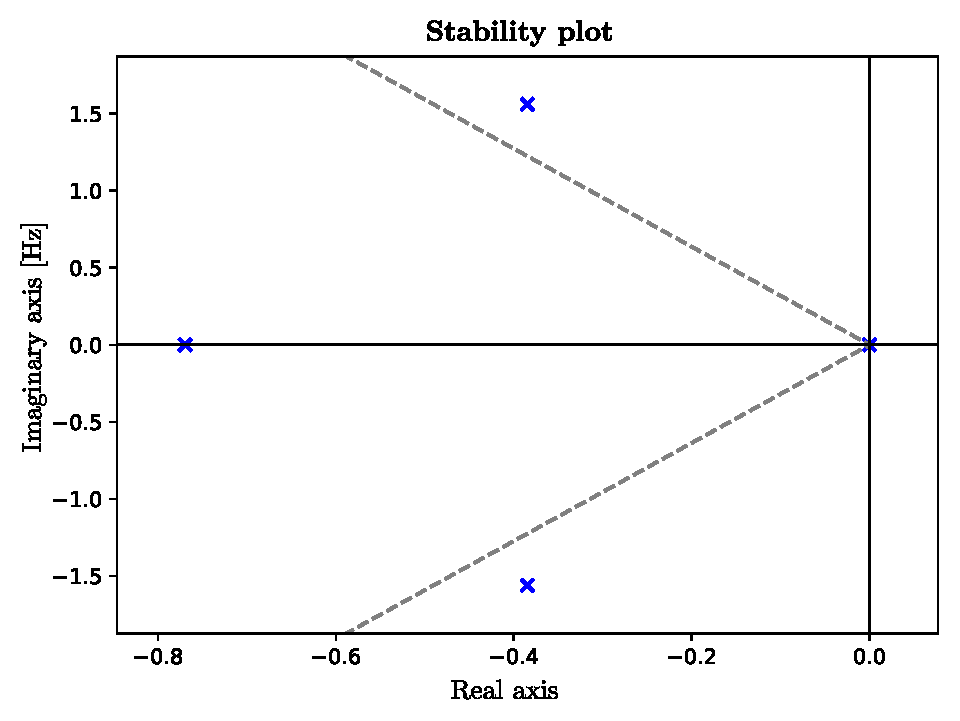
\includegraphics[width=0.8\linewidth]{inkscape_svg/eigenvalues_plot_example.pdf}
  \caption{Eigenvalue plot example.}
  \label{fig:eigenvalues_plot_example}
\end{figure}

The imaginary axis divide the stable part (negative real part) from the unstable part (positive real part). Therefore, all the eigenvalues
represented in the Figure are stable except for one which is in the origin, therefore the system is marginally stable. Moreover, modes outside
the real axis represent oscillatory modes. In this case, one can see that there are
two complex conjugate eigenvalues are represented, which means that the system has an oscillatory mode. the mode in the real axis is a non-oscillatory mode.
Since it is the one with the highest real part, it is the dominant mode of the system.


